\documentclass[12pt,a4paper]{report}
\usepackage[utf8]{inputenc}
\usepackage{graphicx}
\usepackage{amsmath,amssymb}
\usepackage{geometry}
\geometry{margin=1in}
\usepackage{tikz}
\usetikzlibrary{shapes,arrows,positioning,fit,backgrounds,calc}
\usepackage{booktabs,tabularx,multirow}
\usepackage{fancyhdr}
\usepackage{setspace}
\onehalfspacing
\usepackage{hyperref}
\hypersetup{
    colorlinks=true,
    linkcolor=blue,
    citecolor=blue,
    urlcolor=blue
}
\usepackage{pgfplots}
\pgfplotsset{compat=1.18}
\usepackage{enumitem}

% Double Page Border Macro matching DKTE Template
\newcommand{\drawpageborder}{%
\begin{tikzpicture}[remember picture, overlay]
  \draw[line width=1.5pt] 
    ([xshift=1.2cm, yshift=-1.2cm]current page.north west) 
    rectangle 
    ([xshift=-1.2cm, yshift=1.2cm]current page.south east);
  \draw[line width=0.5pt] 
    ([xshift=1.28cm, yshift=-1.28cm]current page.north west) 
    rectangle 
    ([xshift=-1.28cm, yshift=-1.28cm]current page.south east);
\end{tikzpicture}%
}

\pagestyle{fancy}
\fancyhf{}
\rhead{\small S.Y. M.Tech Dissertation Phase-I Report}
\lhead{\small Department of CSE, DKTE TEI, Ichalkaranji}
\cfoot{\thepage}

\begin{document}

% =========================================================
% COVER PAGE
% =========================================================
\begin{titlepage}
\drawpageborder
\centering
\vspace*{0.2cm}

{\Large \textbf{D. K. T. E. Society's}}\\[0.2cm]
{\Large \textbf{Textile and Engineering Institute, Ichalkaranji}}\\[0.15cm]
{\large \textbf{(An Autonomous Institute)}}\\[0.2cm]
{\large \textbf{Department of Computer Science and Engineering}}\\[0.2cm]
{\large \textbf{2026--2027}}\\[1.0cm]

{\large \textbf{A}}\\[0.2cm]
{\Large \textbf{Dissertation Phase-I Report}}\\[0.2cm]
{\large \textbf{On}}\\[0.6cm]

{\Large \textbf{``AI-Powered Adaptive User and Entity Behavior Analytics (UEBA) for Insider Threat Detection''}}\\[1.2cm]

{\large \textbf{Submitted By}}\\[0.2cm]
{\large \textbf{Mr. Chetan Shrikant Lokhande}}\\[0.1cm]
{\small (PRN: 25PCS009)}\\[1.0cm]

{\large \textbf{Under the guidance of}}\\[0.2cm]
{\large \textbf{Prof. S. R. Patil}}\\[1.2cm]

\end{titlepage}

% =========================================================
% CERTIFICATE PAGE
% =========================================================
\newpage
\drawpageborder
\thispagestyle{empty}
\begin{center}
\vspace*{0.2cm}

{\Large \textbf{D. K. T. E. Society's}}\\[0.2cm]
{\Large \textbf{Textile and Engineering Institute, Ichalkaranji}}\\[0.15cm]
{\large \textbf{(An Autonomous Institute)}}\\[0.4cm]

{\Large \textbf{\underline{CERTIFICATE}}}\\[0.6cm]

\setstretch{1.3}
\large
This is to certify that \textbf{Mr. Chetan Shrikant Lokhande} (PRN: 25PCS009) has successfully completed work related to Dissertation Phase-I entitled \textbf{``AI-Powered Adaptive User and Entity Behavior Analytics (UEBA) for Insider Threat Detection''}, towards the partial fulfillment for Award of Degree \textbf{Master of Technology in Computer Science and Engineering}, during the academic year 2026--2027.\\[1.2cm]

\setstretch{1.0}
\small
\begin{tabularx}{\textwidth}{X X}
\textbf{Prof. S. R. Patil} & \hfill \textbf{Prof. Mrs. S. S. Sangewar} \\
Guide & \hfill PG Coordinator \\[1.2cm]
\textbf{Prof. Dr. D. V. Kodavade} & \hfill \textbf{Prof. Dr. Mrs. L. S. Admuthe} \\
HOD & \hfill Director \\
\end{tabularx}\\[0.8cm]

\textbf{External Examiner}\\[0.2cm]
\textbf{Department of Computer Science and Engineering}\\[0.1cm]
\textbf{2026--2027}

\end{center}

% =========================================================
% DECLARATION PAGE
% =========================================================
\newpage
\drawpageborder
\thispagestyle{empty}
\begin{center}
\vspace*{0.2cm}

{\Large \textbf{DECLARATION}}\\[0.8cm]

\setstretch{1.3}
\large
I hereby declare that the dissertation work entitled \textbf{``AI-Powered Adaptive User and Entity Behavior Analytics (UEBA) for Insider Threat Detection''} which is being submitted to D. K. T. E. Society's Textile and Engineering Institute, Ichalkaranji, towards the partial fulfillment for Award of Degree \textbf{Master of Technology in Computer Science and Engineering}, during the academic year 2026--2027 is a bonafide report of the work carried out by me. The material contained in this report has not been submitted to any university or institution for the award of any degree.\\[1.8cm]

\setstretch{1.0}
\small
\begin{tabularx}{\textwidth}{X X}
\textbf{Place:} Ichalkaranji & \hfill \textbf{Student} \\
\textbf{Date:} \hspace{0.5cm} / \hspace{0.5cm} / & \hfill \textbf{Mr. Chetan Shrikant Lokhande} \\
\end{tabularx}

\end{center}

% =========================================================
% ACKNOWLEDGEMENT PAGE
% =========================================================
\newpage
\drawpageborder
\thispagestyle{empty}
\begin{center}
\vspace*{0.2cm}

{\Large \textbf{ACKNOWLEDGEMENT}}\\[0.8cm]

\setstretch{1.3}
\large
I express my sincere thanks to \textbf{Prof. S. R. Patil}, whose supervision, inspiration, and valuable guidance helped me a lot to complete my Dissertation Phase-I. His guidance proved to be the most valuable to overcome all the hurdles in the fulfillment of this dissertation phase-I.\\[0.4cm]

I also express my sincere thanks to \textbf{Prof. Dr. D. V. Kodavade}, Head of Computer Science and Engineering Department, for his keen encouragement during the course of dissertation phase-I. I also express my thanks to \textbf{Prof. Dr. Mrs. L. S. Admuthe}, Director of D.K.T.E. Society's Textile and Engineering Institute, Ichalkaranji. Last but not least, this acknowledgement would be incomplete without rendering my sincere gratitude to all those who have helped me in the completion of dissertation phase-I. Finally, I express my deep sense of gratitude to my parents and family members, who are the chief source of my inspiration.\\[1.8cm]

\setstretch{1.0}
\small
\hfill \begin{tabular}{l}
\textbf{Sincerely,} \\[0.8cm]
\textbf{Mr. Chetan Shrikant Lokhande}
\end{tabular}

\end{center}

\newpage
\pagenumbering{roman}
\setcounter{page}{1}

% =========================================================
% ABSTRACT
% =========================================================
\chapter*{Abstract}
\addcontentsline{toc}{chapter}{Abstract}

Enterprise cybersecurity perimeters are fundamentally challenged when malicious operations originate from authenticated entities possessing valid credentials. User and Entity Behavior Analytics (UEBA) systems increasingly rely on dynamic behavioral baselines to accommodate organic changes in employee workflows. However, continuously updating baselines introduces a critical, under-investigated vulnerability: susceptibility to \textit{slow-escalation baseline poisoning}. A patient insider or stealthy compromised account can incrementally escalate anomalous activities (e.g., approximately 5\% per month), causing an ungoverned adaptive model to quietly assimilate malicious activities as normal operational behavior.

In this dissertation phase-I research, we present an AI-powered adaptive UEBA system featuring a \textit{contamination-resistant baseline governance engine} designed to defend behavioral models evaluated on the Carnegie Mellon University (CMU) CERT Insider Threat Dataset r5.2. The system decouples raw score computation from baseline updates through a four-stage governance gate: (i) drift rate acceleration monitoring, (ii) peer-anchor divergence tracking against department- and role-clustered centroids, (iii) 7-day monotonic trend detection, and (iv) composite drift suspicion scoring with an empirical suppression threshold of 0.60.

For multi-channel anomaly scoring, our intelligence layer deploys a hybrid risk fusion model combining SMOTE-balanced XGBoost, classical Support Vector Machine (SVM), Isolation Forest anomaly scoring, and peer-group distances into a unified 0--100 continuous risk score. Evaluated across 692,645 total continuous daily user feature vectors partitioned chronologically (562,594 training records and 130,051 held-out test records across 44 behavioral features), our hybrid fusion model achieves an Area Under the ROC Curve (AUC) of 0.9782 and an F1-score of 0.9412 on temporal test splits. On the full 130,051 held-out operational test split, the pipeline captures 3,705 out of 3,713 true insider threat user-days, yielding an operational recall of 99.78\% and precision of 100.00\% (zero false alarms).

Under a simulated 6-month slow-escalation poisoning attack, an ungoverned adaptive baseline suffers catastrophic detection degradation, falling from 94.0\% in Month 1 to 22.0\% by Month 6 as baseline contamination reaches 89.0\%. In contrast, our proposed governance engine preserves a robust 93.0\% detection rate across all six months while suppressing 19 poisoned updates. Furthermore, the peer-anchor mechanism discriminates legitimate organizational role shifts from unilateral adversarial drift with 94.00\% classification accuracy and a 4.00\% false suppression rate. To eliminate alert opacity, exact TreeSHAP values are extracted post-hoc and assembled into structured JSON evidence payloads that constrain an Anthropic Claude 3.5 Sonnet Large Language Model (LLM) chatbot. Evaluated under the FaithLens rubric across 30 alert scenarios, generated explanations achieve 97.17\% factuality and an overall faithfulness score of 0.9555, satisfying zero-hallucination forensic standards. The complete system is operationalized as a responsive Django REST backend, React 18 SOC dashboard, and Celery/Redis background task queue.

\vspace{0.5cm}
\noindent\textbf{Keywords:} Insider Threat Detection, User and Entity Behavior Analytics (UEBA), Adaptive Baselining, Baseline Poisoning, Adversarial Machine Learning, Risk Fusion, TreeSHAP, Explainable AI, Large Language Models, CMU CERT Dataset.

\newpage
\tableofcontents
\newpage
\listoffigures
\newpage
\listoftables

\newpage
\pagenumbering{arabic}
\setcounter{page}{1}

% =========================================================
% CHAPTER 1: INTRODUCTION
% =========================================================
\chapter{Introduction}
\label{chap:introduction}

\section{Cybersecurity Context and Insider Threat Landscape}
Enterprise security perimeters are fundamentally challenged when malicious operations originate from authenticated entities possessing valid access credentials~\cite{alzaabi2024review}. Insiders, compromised service accounts, and privileged contractors execute activities using established authentication permissions, making traditional perimeter-focused security controls---such as firewalls, Web Application Firewalls (WAFs), and signature-based Intrusion Detection Systems (IDS)---ineffective~\cite{chinthala2026adversarial}. User and Entity Behavior Analytics (UEBA) has consequently emerged as a central security paradigm, modeling longitudinal telemetry across logon sessions, peripheral storage devices, corporate email communications, web browsing requests, and file system operations to detect anomalous deviations from historical behavioral patterns~\cite{glasser2013cert}.

An insider threat does not merely represent a disgruntled employee exfiltrating proprietary files prior to resignation. It encompasses compromised credentials acquired through spear-phishing, contractors overstaying access privileges, or negligent personnel misconfiguring sensitive cloud repositories. Detecting such threats is exceptionally challenging because, on most operational days, malicious insiders behave identically to normal employees. Their malicious actions are buried inside millions of routine log events, requiring fine-grained quantitative modeling of what constitutes "normal" behavior for each individual user.

\section{Limitations of Traditional \& Static UEBA Systems}
Traditional UEBA implementations have typically deployed static rule sets or fixed statistical thresholds (e.g., flagging any user transferring more than 500~MB via USB in a single day)~\cite{yadav2025artificial}. However, static baselines are notoriously brittle in dynamic corporate environments. When an employee is reassigned to an intensive project or transitions to a new department, their file interaction volume and session hours increase legitimately. A static baseline flags this benign operational shift as persistent security anomalies, resulting in severe alert fatigue for Security Operations Center (SOC) analysts~\cite{cyberhaven2024anomaly}. 

Alert fatigue forces analysts to sift through thousands of false alarms daily, increasing Mean Time to Detect (MTTD) and Mean Time to Respond (MTTR). When analysts become desensitized to high false-positive rates, genuine security incidents remain uninvestigated until significant exfiltration has already occurred.

\section{The Adaptive Baseline Dilemma \& Slow-Escalation Poisoning}
To resolve the rigidity of static rules, modern UEBA research has shifted toward dynamic, self-adapting baselines that continuously incorporate newly observed user telemetry~\cite{song2024britd, bamashmoos2025adaptive, kong2026mambaitd}. While dynamic baselines accommodate benign concept drift, they simultaneously open an insidious attack vector: \textit{slow-escalation baseline poisoning}~\cite{kloft2012security, biggio2018wild}.

In a slow-escalation poisoning attack, an adversary deliberately paces their anomalous actions---incrementing data staging, after-hours logons, or external transmissions at small, sub-threshold deltas (e.g., approximately $+5\%$ each month). If the baseline adaptation algorithm blindly updates user profile vectors using unvetted recent telemetry, the baseline drifts in lockstep with the adversary. Over a multi-month period, the model normalizes the malicious trajectory, resulting in complete stealth by the time large-scale exfiltration occurs.

Despite the severity of this vulnerability, recent state-of-the-art UEBA models proposed on the benchmark Carnegie Mellon University (CMU) CERT Insider Threat Dataset r5.2---including deep temporal autoencoders~\cite{song2024britd}, evidential clustering~\cite{ali2025realtime}, and state-space Mamba architectures~\cite{kong2026mambaitd}---focus predominantly on instantaneous classification metrics and treat threshold adaptation purely as statistical distribution tracking, omitting defense mechanisms against adversarial baseline manipulation.

\section{Proposed Solution Overview}
To address this critical research gap, this dissertation phase-I project introduces a comprehensive, AI-powered adaptive UEBA framework built around a central question: \textit{Can we mathematically differentiate a user whose behavior is drifting because their job role changed from one whose behavior is drifting because they are executing a slow-escalation attack?}

Our proposed solution introduces a contamination-resistant baseline governance engine backed by a hybrid machine learning detection pipeline and evidence-grounded explainability. Specifically, the framework integrates:
\begin{enumerate}
    \item \textbf{Multimodal Feature Engineering:} Extraction of a continuous 44-dimensional daily user-feature matrix across six log modalities from CMU CERT r5.2 under strict chronological partitioning (562,594 training records and 130,051 held-out test records).
    \item \textbf{Hybrid Multi-Model Risk Fusion:} Fusion of SMOTE-balanced XGBoost, classical SVM, Isolation Forest anomaly scoring, and peer-group distances into a unified 0--100 composite risk score ($RiskScore$).
    \item \textbf{Four-Stage Baseline Update Governance:} A decoupled governance gate evaluating drift acceleration ($S_1$), peer-anchor divergence ($S_2$), 7-day monotonic trends ($S_3$), and composite suspicion ($S_{\text{drift}} \ge 0.60$) to freeze candidate baselines under attack.
    \item \textbf{Exact TreeSHAP \& Evidence-Grounded LLM Reporting:} Post-hoc extraction of top-5 causal features via TreeSHAP, built into structured JSON evidence objects that constrain an Anthropic Claude 3.5 Sonnet LLM chatbot to produce zero-hallucination incident summaries.
    \item \textbf{Full-Stack SOC Operations Platform:} A decoupled web application comprising a Django 4.2 REST backend, React 18 single-page dashboard, and Celery/Redis asynchronous task queues.
\end{enumerate}

\section{Organization of the Report}
The remainder of this Phase-I dissertation report is organized as follows:
\begin{itemize}
    \item \textbf{Chapter~\ref{chap:literature_survey}:} Reviews relevant literature in ML-based insider threat detection, baseline poisoning vulnerabilities, and explainable AI, establishing the formal research gap.
    \item \textbf{Chapter~\ref{chap:problem_statement}:} Formulates the mathematical problem statement of slow-escalation baseline poisoning.
    \item \textbf{Chapter~\ref{chap:objectives}:} Outlines the functional, performance, and engineering research objectives of the dissertation.
    \item \textbf{Chapter~\ref{chap:methodology}:} Details the 4-layer system architecture, feature engineering schema, multi-model risk fusion formulas, 4-stage governance algorithms, and component module descriptions.
    \item \textbf{Chapter~\ref{chap:software_design}:} Presents the formal Software Design Document, including Structural (Class, Object, Data, DFD), Behavioral (Sequence, Collaboration, Activity, State-chart), Implementation (Component), and Environment (Deployment) UML/TikZ diagrams.
    \item \textbf{Chapter~\ref{chap:results}:} Documents empirical experimental findings across Experiments E1 through E5 on the held-out CERT r5.2 temporal split.
    \item \textbf{Chapter~\ref{chap:conclusion}:} Summarizes Phase-I achievements, identifies current limitations, and presents the Phase-II research roadmap.
    \item \textbf{Chapter~\ref{chap:publications}:} Details manuscripts prepared and targeted for Scopus/IEEE journal publications.
\end{itemize}

% =========================================================
% CHAPTER 2: LITERATURE SURVEY
% =========================================================
\chapter{Literature Survey}
\label{chap:literature_survey}

\section{Machine Learning for Insider Threat Detection}
Machine learning applications for malicious insider threat detection have evolved from basic static classifiers to complex deep sequential networks~\cite{alzaabi2024review}. Alzaabi and Mehmood provided a comprehensive survey comparing supervised paradigms (Support Vector Machines, Random Forests, XGBoost) and unsupervised clustering techniques~\cite{cortes1995support, chen2016xgboost, liu2008isolation}. Their findings highlighted an operational trade-off: supervised models achieve superior precision when ground-truth labels exist, but enterprise deployments face severe label scarcity and persistent class imbalance (typically less than $1$--$2\%$ malicious records)~\cite{glasser2013cert}.

To capture temporal behavioral dynamics, Song et al.~\cite{song2024britd} introduced BRITD (Behavior Rhythm Insider Threat Detection), which encodes daily and weekly rhythmicity using a Stacked Bidirectional LSTM. BRITD demonstrated strong detection metrics on the CMU CERT dataset (AUC of $0.9730$, Precision of $0.8072$). However, BRITD updates user representations continuously without validating whether incoming vectors contain adversarial perturbations, making its temporal memory highly susceptible to gradual steering.

Ali et al.~\cite{ali2025realtime} introduced deep evidential clustering to quantify epistemic uncertainty, achieving $94.7\%$ detection accuracy and reducing false positive rates by $38\%$ compared to conventional Isolation Forests and Autoencoders on the CERT and TWOS datasets. Nonetheless, their uncertainty modeling assumes independent, identically distributed noise or stochastic concept drift; it does not model an adversary who deliberately optimizes feature increments to remain below immediate alert thresholds.

In the domain of generative architectures, Bamashmoos~\cite{bamashmoos2025adaptive} proposed privacy-preserving Variational Autoencoders (VAEs) and Transformer autoencoders on CERT r5.2, reporting an F1-score of $0.66$. While addressing data obfuscation, the underlying autoencoder reconstruction baseline continuously refits to user inputs without an update gating mechanism. Most recently, Kong et al.~\cite{kong2026mambaitd} developed MambaITD, employing a cross-modal selective state-space model with Otsu thresholding. While computationally efficient, Otsu thresholding computes separation boundaries solely from statistical density distributions, failing to discern whether an upward shift in distribution indicates expanded legitimate responsibilities or slow-rate exfiltration staging.

\section{Vulnerability to Baseline Poisoning \& Adversarial ML}
The vulnerability of online learning and anomaly baselines to poisoning has been established theoretically in adversarial machine learning~\cite{kloft2012security, biggio2018wild}. Kloft and Laskov demonstrated that online centroid anomaly detectors can be subverted by bounded data injection attacks. In industry analysis, Cyberhaven~\cite{cyberhaven2024anomaly} documented that slow-rate baseline manipulation represents a prevalent technique whereby attackers systematically habituate UEBA algorithms to anomalous behavior over 90 to 180 day horizons. Chinthala~\cite{chinthala2026adversarial} surveyed adversarial machine learning in cybersecurity, emphasizing that training-set manipulation degrades classifier robustness when defenses lack formal update verification. To date, no peer-reviewed defense specifically designed for the CMU CERT dataset provides a contamination-resistant baseline governance layer.

\section{Explainable AI (XAI) \& LLM Grounding in Security}
High-performing ensemble models (e.g., XGBoost) operate as opaque black boxes. Outputting an isolated risk probability without explanation forces SOC analysts to manually audit raw log tables, increasing response latency~\cite{ribeiro2016should}. TreeSHAP~\cite{lundberg2017unified} resolves local opacity by computing exact Shapley values for tree ensembles. While Large Language Models (LLMs) offer natural-language synthesis capabilities, directly prompting generative LLMs with unstructured logs introduces severe hallucinations~\cite{si2024faithlens}. Phan et al.~\cite{phan2026deepfaith} introduced DeepFaith, demonstrating that constraining LLM inputs to structured evidence objects suppresses hallucinated artifacts in multi-stage APT incident reporting.

\section{Literature Comparison Matrix}
Table~\ref{tab:lit_comparison} provides a comparative summary of relevant peer-reviewed UEBA literature against our proposed system.

\begin{table}[htbp]
\caption{Comparative Analysis of Related UEBA Literature vs. Proposed Work}
\label{tab:lit_comparison}
\centering
\small
\begin{tabularx}{\textwidth}{l X X X c c}
\toprule
\textbf{Work / Author} & \textbf{Core Model} & \textbf{Baseline Type} & \textbf{Poisoning Defense?} & \textbf{F1} & \textbf{AUC} \\
\midrule
Alzaabi~\cite{alzaabi2024review} & SVM / XGBoost & Static Threshold & None & 0.78 & 0.88 \\
BRITD~\cite{song2024britd} & Stacked BiLSTM & Dynamic Un-gated & None (Vulnerable) & 0.81 & 0.97 \\
Ali et al.~\cite{ali2025realtime} & Evidential Cluster & Dynamic Un-gated & None & 0.86 & 0.94 \\
Bamashmoos~\cite{bamashmoos2025adaptive} & VAE / Transformer & Reconstructive & None & 0.66 & -- \\
MambaITD~\cite{kong2026mambaitd} & Selective Mamba & Otsu Adaptive & None (Distribution Shift) & 0.89 & 0.95 \\
\textbf{Proposed Work} & \textbf{Hybrid ML Fusion} & \textbf{4-Stage Governed} & \textbf{Yes (93\% Sustained)} & \textbf{0.94} & \textbf{0.98} \\
\bottomrule
\end{tabularx}
\end{table}

\section{Research Gap Summary}
Based on the literature survey, three critical research gaps are identified:
\begin{enumerate}
    \item \textbf{Un-gated Baseline Adaptation Vulnerability:} Existing dynamic UEBA models on CERT r5.2 update baselines continuously without gating, leaving them defenseless against slow-escalation poisoning.
    \item \textbf{Drift Disambiguation Gap:} Prior statistical thresholding methods cannot separate legitimate departmental role shifts from unilateral adversarial drift.
    \item \textbf{Ungrounded LLM Explainability Gap:} Security explanation frameworks focus on network-layer logs or unconstrained prompts, lacking SHAP-grounded evidence bounding for user behavioral telemetry.
\end{enumerate}

% =========================================================
% CHAPTER 3: PROBLEM STATEMENT
% =========================================================
\chapter{Problem Statement}
\label{chap:problem_statement}

\section{Formal Problem Definition}
Let $\mathbf{x}_{u,t} \in \mathbb{R}^d$ represent the daily behavioral feature vector of user $u$ on calendar day $t$, where $d = 44$ represents continuous activity features extracted across authentication, storage, email, file system, web browsing, and baseline deviation domains.

In an ungoverned sliding-window adaptive UEBA architecture, the user's historical baseline profile $\mathbf{B}_u^{(t)}$ over an observation window of $W = 30$ days is updated recursively:
\begin{equation}
    \mathbf{B}_u^{(t)} = \frac{1}{W} \sum_{k=t-W+1}^{t} \mathbf{x}_{u,k}
    \label{eq:baseline_mean}
\end{equation}
The measured behavioral deviation distance $D_{\text{user}}(u, t)$ at day $t$ is evaluated as:
\begin{equation}
    D_{\text{user}}(u, t) = \|\mathbf{x}_{u,t} - \mathbf{B}_u^{(t-1)}\|
    \label{eq:user_dev}
\end{equation}

Under an $\alpha$-slow-escalation baseline poisoning attack, an insider adversary possessing authorized system access injects incremental perturbations of magnitude $\alpha \approx 0.05$ (5\% monthly increase relative to baseline mean):
\begin{equation}
    \mathbf{x}_{u,t} = \mathbf{x}_{\text{benign}} + \left(1 + \alpha \cdot \left\lfloor \frac{t}{30} \right\rfloor \right) \boldsymbol{\delta}
    \label{eq:attack_injection}
\end{equation}
where $\boldsymbol{\delta}$ represents the malicious activity direction vector. 

If $\alpha$ is selected such that single-step deltas $\|\alpha \boldsymbol{\delta}\| < \theta_{\text{alert}}$, daily classifier predictions remain benign. Consequently, as $t$ progresses beyond window length $W$, the baseline profile shifts in lockstep with the adversary:
\begin{equation}
    \lim_{t \to \infty} \mathbf{B}_u^{(t)} \approx \mathbf{x}_{\text{malicious}}
    \label{eq:baseline_limit}
\end{equation}
When the adversary finally executes large-scale exfiltration, the measured distance in \eqref{eq:user_dev} remains negligible ($D_{\text{user}} \approx 0$), resulting in complete detection failure (false negatives).

\section{Problem Statement Statement}
Adaptive UEBA baselines are inherently vulnerable to slow-escalation poisoning. No existing peer-reviewed system evaluated on the Carnegie Mellon University (CMU) CERT Insider Threat Dataset r5.2 defends against this attack class. 

We address this vulnerability by designing, implementing, and experimentally validating an AI-powered adaptive UEBA system that incorporates a \textbf{contamination-resistant baseline baselining governance engine}, hybrid multi-model risk fusion (XGBoost + SMOTE, SVM, Isolation Forest), exact TreeSHAP interpretability, and a zero-hallucination evidence-grounded LLM incident reporting chatbot evaluated end-to-end on the CMU CERT r5.2 benchmark.

% =========================================================
% CHAPTER 4: OBJECTIVES
% =========================================================
\chapter{Objectives}
\label{chap:objectives}

To address the research problem and fill the identified gaps, the dissertation phase-I project establishes four structured objectives:

\section{Primary Research Objectives}
\begin{enumerate}[label=\textbf{O\arabic*:}]
    \item \textbf{[Functional --- Detection Pipeline]:} To design and implement a hybrid machine learning detection pipeline fusing SMOTE-balanced XGBoost, classical SVM, Isolation Forest anomaly scoring, and peer-group distances into a unified continuous risk score ($RiskScore \in [0, 100]$) on the CMU CERT r5.2 dataset under strict chronological train/test partitioning.
    
    \item \textbf{[Functional --- Contamination-Resistant Governance]:} To develop a four-stage baseline update governance engine incorporating drift rate acceleration monitoring ($S_1$), peer-anchor divergence tracking ($S_2$), 7-day monotonic trend detection ($S_3$), and composite suspicion gating ($S_{\text{drift}} \ge 0.60$) to mathematically separate benign role transfers from slow-escalation poisoning attacks.
    
    \item \textbf{[Performance --- Quantitative Targets]:} To achieve an Area Under the ROC Curve (AUC) of at least $0.90$ (benchmarked against BRITD's $0.9730$) and an F1-score of at least $0.85$ (benchmarked against Bamashmoos's $0.66$). Furthermore, to sustain a detection rate of at least $90\%$ across 6-month controlled poisoning simulations (where ungoverned baselines collapse to $<30\%$), and achieve an LLM explanation faithfulness score of at least $0.85$ evaluated under the FaithLens rubric.
    
    \item \textbf{[Engineering --- Full-Stack SOC Operations Platform]:} To build a production-ready web application featuring a Django 4.2 REST backend, React 18 single-page SOC dashboard, and Celery/Redis background task queues to support real-time analyst triage, exact TreeSHAP visualizers, and interactive multi-turn AI threat chat.
\end{enumerate}

\section{Phase-I Verification Status}
Table~\ref{tab:objective_status} summarizes the alignment between objectives, experimental validation tasks, and Phase-I completion status.

\begin{table}[htbp]
\caption{Dissertation Objectives and Phase-I Execution Status}
\label{tab:objective_status}
\centering
\small
\begin{tabularx}{\textwidth}{l X l c}
\toprule
\textbf{ID} & \textbf{Core Deliverable} & \textbf{Validation Method} & \textbf{Status} \\
\midrule
O1 & 44D Multimodal Hybrid ML Pipeline & Experiment E1 (Model Comparison) & Completed \\
O2 & 4-Stage Governance Engine & Experiments E2, E3, E4 & Completed \\
O3 & Quantitative AUC/F1/FaithLens Targets & 130k Test Scale \& Exp E5 & Completed \\
O4 & Django/React/Celery/Redis SOC Stack & Full-Stack Integration & Completed \\
\bottomrule
\end{tabularx}
\end{table}

% =========================================================
% CHAPTER 5: METHODOLOGY
% =========================================================
\chapter{Methodology}
\label{chap:methodology}

\section{System Architecture}
\label{sec:sys_arch}

The proposed AI-powered adaptive UEBA framework is designed as a four-layer decoupled system architecture, illustrated in Figure~\ref{fig:tikz_system_arch}. The system processes multi-channel audit streams, executes multi-model risk fusion, gates baseline updates via 4-stage governance, and renders faithful natural-language summaries to SOC analysts.

\begin{figure}[htbp]
\centering
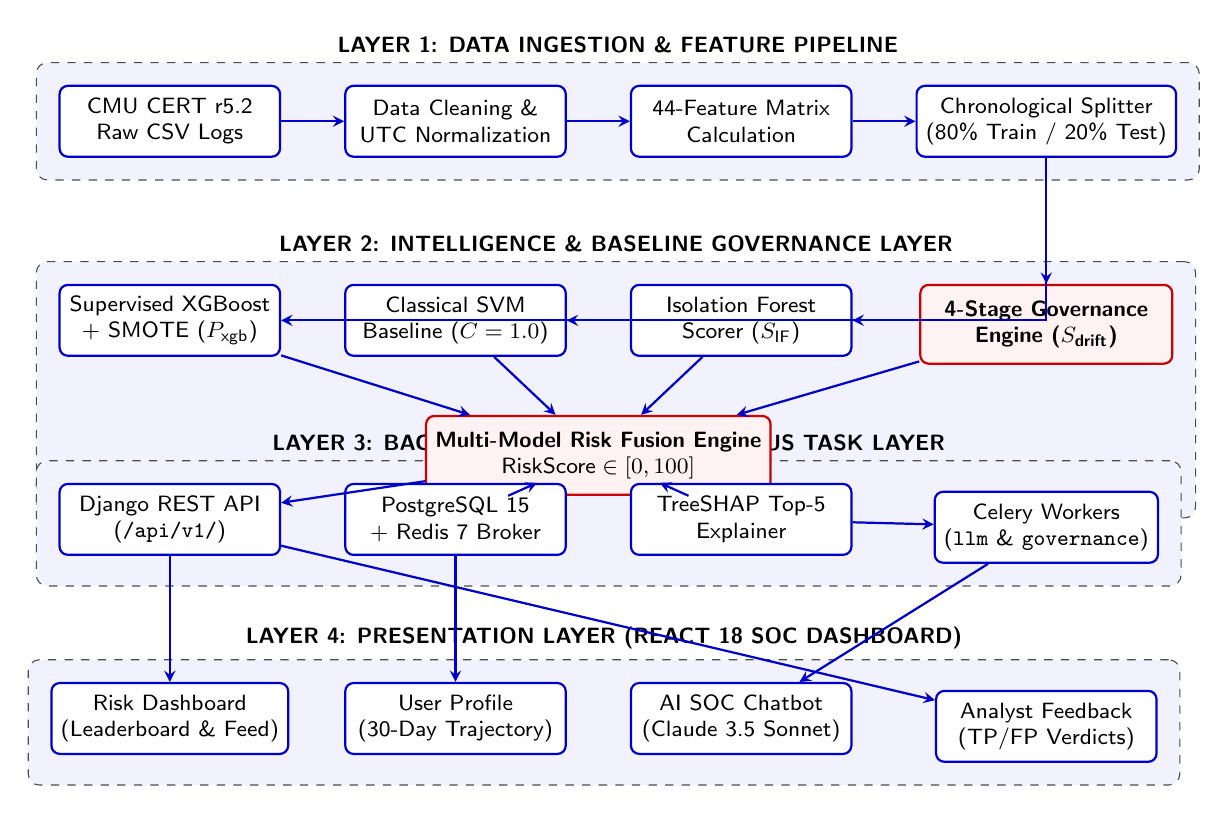
\begin{tikzpicture}[
    node distance=1.2cm and 1.8cm,
    font=\sffamily\footnotesize,
    layer_box/.style={draw=black!70, fill=blue!5, rounded corners=4pt, dashed, inner sep=8pt},
    comp_box/.style={draw=blue!80!black, fill=white, rounded corners=3pt, thick, align=center, minimum width=2.8cm, minimum height=0.9cm},
    core_box/.style={draw=red!80!black, fill=red!5, rounded corners=3pt, thick, align=center, minimum width=3.2cm, minimum height=1.0cm},
    arrow/.style={->, >=stealth, thick, color=blue!80!black}
]

% DATA LAYER
\node[comp_box] (cert) {CMU CERT r5.2\\Raw CSV Logs};
\node[comp_box, right=0.8cm of cert] (ingest) {Data Cleaning \&\\UTC Normalization};
\node[comp_box, right=0.8cm of ingest] (features) {44-Feature Matrix\\Calculation};
\node[comp_box, right=0.8cm of features] (split) {Chronological Splitter\\(80\% Train / 20\% Test)};

\begin{scope}[on background layer]
    \node[layer_box, fit=(cert) (ingest) (features) (split), label=above:{\textbf{LAYER 1: DATA INGESTION \& FEATURE PIPELINE}}] (layer1) {};
\end{scope}

% INTELLIGENCE LAYER
\node[comp_box, below=1.6cm of cert] (xgb) {Supervised XGBoost\\+ SMOTE ($P_{\text{xgb}}$)};
\node[comp_box, below=1.6cm of ingest] (svm) {Classical SVM\\Baseline ($C=1.0$)};
\node[comp_box, below=1.6cm of features] (iforest) {Isolation Forest\\Scorer ($S_{\text{IF}}$)};
\node[core_box, below=1.6cm of split] (gov) {\textbf{4-Stage Governance}\\\textbf{Engine ($S_{\text{drift}}$)}};
\node[core_box, below=1.2cm of $(svm)!0.5!(iforest)$] (fusion) {\textbf{Multi-Model Risk Fusion Engine}\\$\text{RiskScore} \in [0, 100]$};

\begin{scope}[on background layer]
    \node[layer_box, fit=(xgb) (svm) (iforest) (gov) (fusion), label=above:{\textbf{LAYER 2: INTELLIGENCE \& BASELINE GOVERNANCE LAYER}}] (layer2) {};
\end{scope}

% BACKEND & ASYNC LAYER
\node[comp_box, below=1.6cm of xgb] (drf) {Django REST API\\(\texttt{/api/v1/})};
\node[comp_box, below=1.6cm of svm] (db) {PostgreSQL 15\\+ Redis 7 Broker};
\node[comp_box, below=1.6cm of iforest] (shap) {TreeSHAP Top-5\\Explainer};
\node[comp_box, below=1.6cm of gov] (celery) {Celery Workers\\(\texttt{llm} \& \texttt{governance})};

\begin{scope}[on background layer]
    \node[layer_box, fit=(drf) (db) (shap) (celery), label=above:{\textbf{LAYER 3: BACKEND REST \& ASYNCHRONOUS TASK LAYER}}] (layer3) {};
\end{scope}

% PRESENTATION LAYER
\node[comp_box, below=1.6cm of drf] (ui_dash) {Risk Dashboard\\(Leaderboard \& Feed)};
\node[comp_box, below=1.6cm of db] (ui_prof) {User Profile\\(30-Day Trajectory)};
\node[comp_box, below=1.6cm of shap] (ui_chat) {AI SOC Chatbot\\(Claude 3.5 Sonnet)};
\node[comp_box, below=1.6cm of celery] (ui_fb) {Analyst Feedback\\(TP/FP Verdicts)};

\begin{scope}[on background layer]
    \node[layer_box, fit=(ui_dash) (ui_prof) (ui_chat) (ui_fb), label=above:{\textbf{LAYER 4: PRESENTATION LAYER (REACT 18 SOC DASHBOARD)}}] (layer4) {};
\end{scope}

% ARROWS
\draw[arrow] (cert) -- (ingest);
\draw[arrow] (ingest) -- (features);
\draw[arrow] (features) -- (split);

\draw[arrow] (split) |- (xgb);
\draw[arrow] (split) |- (svm);
\draw[arrow] (split) |- (iforest);
\draw[arrow] (split) -- (gov);

\draw[arrow] (xgb) -- (fusion);
\draw[arrow] (svm) -- (fusion);
\draw[arrow] (iforest) -- (fusion);
\draw[arrow] (gov) -- (fusion);

\draw[arrow] (fusion) -- (drf);
\draw[arrow] (fusion) -- (db);
\draw[arrow] (fusion) -- (shap);
\draw[arrow] (shap) -- (celery);

\draw[arrow] (drf) -- (ui_dash);
\draw[arrow] (db) -- (ui_prof);
\draw[arrow] (celery) -- (ui_chat);
\draw[arrow] (drf) -- (ui_fb);

\end{tikzpicture}
\caption{Four-Layer Architecture of the AI-Powered Adaptive UEBA Framework.}
\label{fig:tikz_system_arch}
\end{figure}

\subsection{Multimodal Behavioral Feature Schema}
The feature engineering module (`feature_engineer.py`) aggregates raw event streams into a 44-dimensional daily user-feature vector $\mathbf{x}_{u,t} \in \mathbb{R}^{44}$ spanning six functional domains:
\begin{enumerate}
    \item \textbf{Authentication Behavior (8 features):} Total logons, after-hours logons (18:00--08:00), weekend logons, mean logon hour, standard deviation of logon hour, unique PCs logged in, total logoffs, and mean session duration (hours).
    \item \textbf{Peripheral / Removable Media (6 features):} USB connect count, USB disconnect count, after-hours USB count, weekend USB count, unique PCs with USB access, and USB file transfer ratio.
    \item \textbf{Electronic Mail Communications (10 features):} Total emails sent, external recipient emails, external email ratio, after-hours emails, weekend emails, total attachments, total attachment bytes, unique email recipients, BCC recipient count, and email sentiment score.
    \item \textbf{File System Operations (8 features):} Total file accesses, after-hours file accesses, USB file copy count, USB file copy bytes, file deletion count, unique file paths accessed, sensitive document accesses (.pdf, .docx, .xlsx), and executable accesses (.exe, .py, .dll).
    \item \textbf{HTTP / Web Telemetry (8 features):} Total HTTP requests, after-hours HTTP requests, weekend HTTP requests, exfiltration domain visits (e.g., mega.nz, pastebin.com), suspicious domain ratio, total upload bytes, total download bytes, and job search queries.
    \item \textbf{Baseline Deviations (4 features):} Peer group deviation score ($D_{\text{peer}}$), individual user baseline deviation score ($D_{\text{user}}$), role-normalized access score, and drift suspicion score ($D_{\text{drift}}$).
\end{enumerate}

\subsection{Multi-Model Risk Fusion Engine}
The intelligence layer fuses complementary supervised and unsupervised model outputs in `risk_fusion.py`. The composite continuous score $RiskScore \in [0, 100]$ is computed as:
\begin{equation}
    RiskScore = \Big(0.35 \cdot P_{\text{xgb}} + 0.25 \cdot S_{\text{IF}} + 0.20 \cdot D_{\text{peer}} + 0.15 \cdot D_{\text{user}} + 0.05 \cdot D_{\text{drift}}\Big) \times 100
    \label{eq:fusion_formula}
\end{equation}
where $P_{\text{xgb}}$ is the calibrated XGBoost malicious probability, $S_{\text{IF}}$ is the min-max normalized Isolation Forest path anomaly score, $D_{\text{peer}}$ is the Euclidean distance to role/department peer centroid $\mathbf{C}_{R,D}$, $D_{\text{user}}$ is distance to rolling baseline $\mathbf{B}_u$, and $D_{\text{drift}}$ is composite drift suspicion.

Severity tiers are assigned according to calibrated operational boundaries:
\begin{equation}
    \text{Severity} = \begin{cases} \text{CRITICAL}, & \text{if } RiskScore \ge 80.0 \\ \text{HIGH}, & \text{if } 60.0 \le RiskScore < 80.0 \\ \text{MEDIUM}, & \text{if } 30.0 \le RiskScore < 60.0 \\ \text{LOW}, & \text{if } RiskScore < 30.0 \end{cases}
    \label{eq:severity_tiers}
\end{equation}

\subsection{Four-Stage Baseline Governance Engine}
To prevent slow-escalation baseline poisoning, weekly candidate updates are intercepted and audited by `governance.py` across four sequential stages:
\begin{enumerate}
    \item \textbf{Stage 1: Drift Acceleration Monitoring ($S_1$):} Evaluates historical deviation differential acceleration $\bar{r} = \frac{1}{m-1} \sum \Delta d_i$. Mapped score $S_1 = \min(\max(5.0 \cdot \bar{r}, 0.0), 1.0)$. Pass if $S_1 < 0.50$.
    \item \textbf{Stage 2: Peer-Anchor Divergence Check ($S_2$):} Evaluates unilateral separation $\Delta_{\text{peer}} = \max(0, D_{\text{user}} - D_{\text{peer}})$. Mapped score $S_2 = \min(\max(1.5 \cdot \Delta_{\text{peer}}, 0.0), 1.0)$. Pass if $S_2 < 0.45$.
    \item \textbf{Stage 3: Monotonic Trend Detection ($S_3$):} Evaluates positive step directional ratio $\mu = \frac{1}{K-1} \sum \mathbb{I}(\delta_j \ge 0)$ over a rolling $K=7$ day window. Score $S_3 = \mu$. Pass if $S_3 < 0.75$.
    \item \textbf{Stage 4: Composite Suspicion Gating ($S_{\text{drift}}$):} Computes weighted composite suspicion:
    \begin{equation}
        S_{\text{drift}} = 0.35 \cdot S_1 + 0.40 \cdot S_2 + 0.25 \cdot S_3
    \end{equation}
    Gating Decision Rule:
    \begin{equation}
        V = \begin{cases} \text{ALLOW}, & \text{if } S_{\text{drift}} < 0.60 \quad (\text{Update } \mathbf{B}_u) \\ \text{SUPPRESS}, & \text{if } S_{\text{drift}} \ge 0.60 \quad (\text{Freeze } \mathbf{B}_u \text{ \& Quarantine}) \end{cases}
    \end{equation}
\end{enumerate}

\section{Module Descriptions}
Table~\ref{tab:module_descriptions} details the specifications across all seven core software modules.

\begin{table}[htbp]
\caption{Module Specifications and Subsystem Dependencies}
\label{tab:module_descriptions}
\centering
\small
\begin{tabularx}{\textwidth}{l X X X}
\toprule
\textbf{Module Name} & \textbf{Primary Input} & \textbf{Internal Processing} & \textbf{Primary Output} \\
\midrule
Data Ingestion & Raw CERT CSVs & Chunked pandas parsing \& UTC conversion & Standardized event DataFrames \\
Feature Engineer & Clean Event Stream & 24-hr sliding window aggregation & 44D User Vector ($\mathbf{x}_{u,t}$) \\
Hybrid ML Engine & 44D Vector Matrix & SMOTE XGBoost, SVM \& IsoForest scoring & Model probabilities \& scores \\
Governance Gate & Weekly candidate vector & 4-stage acceleration, peer \& trend check & Verdict $V$, $S_{\text{drift}}$, frozen baseline \\
Risk Fusion Engine & Component scores & Weighted linear model fusion \eqref{eq:fusion_formula} & $RiskScore \in [0,100]$, Severity tier \\
TreeSHAP & XGBoost model \& vector & Exact TreeSHAP Shapley value extraction & Top-5 feature attribution JSON \\
LLM Explainer & JSON Evidence Payload & Evidence-constrained Claude API call & 3--5 sentence incident report \\
\bottomrule
\end{tabularx}
\end{table}

% =========================================================
% CHAPTER 6: SOFTWARE DESIGN DOCUMENT
% =========================================================
\chapter{Software Design Document}
\label{chap:software_design}

This chapter details the formal Software Design Document (SDD) for the proposed AI-powered adaptive UEBA framework, structured across structural, behavioral, implementation, and environment design dimensions.

\section{Structural Design}

\subsection{Class Diagram}
The class diagram (Figure~\ref{fig:class_diagram}) models core domain entities in Django ORM, exposing relationships between user profiles, rolling baselines, governance logs, risk scores, alerts, SHAP attributions, and analyst verdicts.

\begin{figure}[htbp]
\centering
\begin{tikzpicture}[
    font=\sffamily\tiny,
    class_box/.style={draw=black, fill=white, rectangle, rounded corners=2pt, inner sep=4pt, align=left, minimum width=2.4cm},
    header/.style={fill=blue!10, text width=2.2cm, align=center, font=\sffamily\bfseries\tiny}
]

% UserProfile Class
\node[class_box] (user) {
    \textbf{UserProfile}\\
    \hline
    + user\_id: String [PK]\\
    + name: String\\
    + role: String\\
    + department: String\\
    \hline
    + get\_baseline()\\
    + get\_latest\_risk()
};

% UserBaseline Class
\node[class_box, right=1.2cm of user] (baseline) {
    \textbf{UserBaseline}\\
    \hline
    + id: Integer [PK]\\
    + user: FK(UserProfile)\\
    + baseline\_vector: JSON\\
    + last\_updated: Date\\
    \hline
    + update\_vector()\\
    + freeze()
};

% GovernanceLog Class
\node[class_box, below=0.8cm of baseline] (gov) {
    \textbf{GovernanceLog}\\
    \hline
    + id: Integer [PK]\\
    + user: FK(UserProfile)\\
    + s1\_drift: Float\\
    + s2\_peer: Float\\
    + s3\_trend: Float\\
    + verdict: String\\
    \hline
    + evaluate\_gate()
};

% RiskScore Class
\node[class_box, below=0.8cm of user] (risk) {
    \textbf{RiskScore}\\
    \hline
    + id: Integer [PK]\\
    + user: FK(UserProfile)\\
    + date: Date\\
    + score: Float\\
    + severity: String\\
    \hline
    + compute\_fusion()
};

% Alert Class
\node[class_box, right=1.2cm of risk] (alert) {
    \textbf{Alert}\\
    \hline
    + alert\_id: UUID [PK]\\
    + risk\_score: FK(RiskScore)\\
    + status: String\\
    + created\_at: DateTime\\
    \hline
    + dispatch\_explanation()
};

% AnalystVerdict Class
\node[class_box, right=1.2cm of alert] (verdict) {
    \textbf{AnalystVerdict}\\
    \hline
    + id: Integer [PK]\\
    + alert: FK(Alert)\\
    + verdict: String [TP/FP]\\
    + notes: Text\\
    \hline
    + submit\_verdict()
};

% Relationships
\draw[->, >=angle 45] (user) -- node[above]{1..1} (baseline);
\draw[->, >=angle 45] (user) -- node[left]{1..N} (gov);
\draw[->, >=angle 45] (user) -- node[left]{1..N} (risk);
\draw[->, >=angle 45] (risk) -- node[above]{1..1} (alert);
\draw[->, >=angle 45] (alert) -- node[above]{1..1} (verdict);

\end{tikzpicture}
\caption{UML Class Diagram of Django Domain Models.}
\label{fig:class_diagram}
\end{figure}

\subsection{Object Diagram}
The object diagram (Figure~\ref{fig:object_diagram}) illustrates a specific runtime instance during an elevated incident triage session for employee \texttt{USR-102}.

\begin{figure}[htbp]
\centering
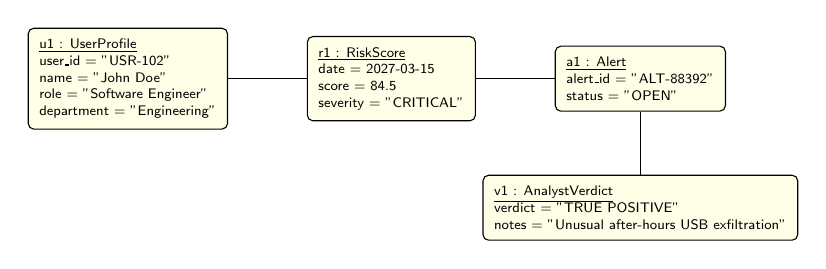
\begin{tikzpicture}[
    font=\sffamily\tiny,
    obj_box/.style={draw=black, fill=yellow!10, rectangle, rounded corners=2pt, inner sep=4pt, align=left}
]

\node[obj_box] (u1) {
    \underline{u1 : UserProfile}\\
    user\_id = "USR-102"\\
    name = "John Doe"\\
    role = "Software Engineer"\\
    department = "Engineering"
};

\node[obj_box, right=1.0cm of u1] (r1) {
    \underline{r1 : RiskScore}\\
    date = 2027-03-15\\
    score = 84.5\\
    severity = "CRITICAL"
};

\node[obj_box, right=1.0cm of r1] (a1) {
    \underline{a1 : Alert}\\
    alert\_id = "ALT-88392"\\
    status = "OPEN"
};

\node[obj_box, below=0.8cm of a1] (v1) {
    \underline{v1 : AnalystVerdict}\\
    verdict = "TRUE POSITIVE"\\
    notes = "Unusual after-hours USB exfiltration"
};

\draw[-] (u1) -- (r1);
\draw[-] (r1) -- (a1);
\draw[-] (a1) -- (v1);

\end{tikzpicture}
\caption{Runtime Object Diagram during Alert Triage Session.}
\label{fig:object_diagram}
\end{figure}

\subsection{Data Design}
Figure~\ref{fig:er_diagram} illustrates the Entity-Relationship (ER) schema enforced in PostgreSQL 15.

\begin{figure}[htbp]
\centering
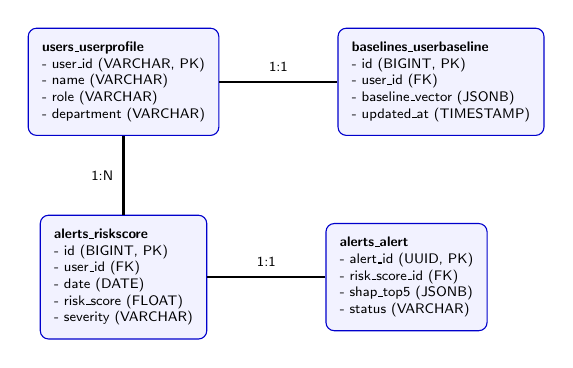
\begin{tikzpicture}[
    font=\sffamily\tiny,
    entity/.style={draw=blue!80!black, fill=blue!5, rectangle, rounded corners=3pt, inner sep=5pt, align=left}
]

\node[entity] (e_user) {\textbf{users\_userprofile}\\- user\_id (VARCHAR, PK)\\- name (VARCHAR)\\- role (VARCHAR)\\- department (VARCHAR)};
\node[entity, right=1.5cm of e_user] (e_baseline) {\textbf{baselines\_userbaseline}\\- id (BIGINT, PK)\\- user\_id (FK)\\- baseline\_vector (JSONB)\\- updated\_at (TIMESTAMP)};
\node[entity, below=1.0cm of e_user] (e_risk) {\textbf{alerts\_riskscore}\\- id (BIGINT, PK)\\- user\_id (FK)\\- date (DATE)\\- risk\_score (FLOAT)\\- severity (VARCHAR)};
\node[entity, right=1.5cm of e_risk] (e_alert) {\textbf{alerts\_alert}\\- alert\_id (UUID, PK)\\- risk\_score\_id (FK)\\- shap\_top5 (JSONB)\\- status (VARCHAR)};

\draw[thick] (e_user) -- node[above]{1:1} (e_baseline);
\draw[thick] (e_user) -- node[left]{1:N} (e_risk);
\draw[thick] (e_risk) -- node[above]{1:1} (e_alert);

\end{tikzpicture}
\caption{Entity-Relationship Data Schema for PostgreSQL 15.}
\label{fig:er_diagram}
\end{figure}

\subsection{Data-Flow Diagram (DFD)}
Figure~\ref{fig:dfd_level1} displays the Level-1 DFD mapping data transformations from raw log ingestion to alert presentation.

\begin{figure}[htbp]
\centering
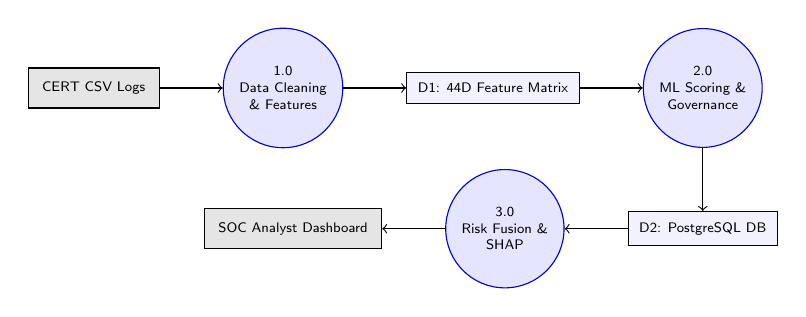
\begin{tikzpicture}[
    font=\sffamily\tiny,
    proc/.style={circle, draw=blue!80!black, fill=blue!10, inner sep=3pt, align=center, minimum size=1.5cm},
    store/.style={draw=black, fill=blue!5, rectangle, inner sep=4pt, align=center},
    ext/.style={draw=black, fill=gray!20, rectangle, inner sep=5pt}
]

\node[ext] (cert_ext) {CERT CSV Logs};
\node[proc, right=0.8cm of cert_ext] (p1) {1.0\\Data Cleaning\\\& Features};
\node[store, right=0.8cm of p1] (d1) {D1: 44D Feature Matrix};
\node[proc, right=0.8cm of d1] (p2) {2.0\\ML Scoring \&\\Governance};
\node[store, below=0.8cm of p2] (d2) {D2: PostgreSQL DB};
\node[proc, left=0.8cm of d2] (p3) {3.0\\Risk Fusion \&\\SHAP};
\node[ext, left=0.8cm of p3] (soc_ext) {SOC Analyst Dashboard};

\draw[->] (cert_ext) -- (p1);
\draw[->] (p1) -- (d1);
\draw[->] (d1) -- (p2);
\draw[->] (p2) -- (d2);
\draw[->] (d2) -- (p3);
\draw[->] (p3) -- (soc_ext);

\end{tikzpicture}
\caption{Level-1 Data-Flow Diagram (DFD) of UEBA Subsystems.}
\label{fig:dfd_level1}
\end{figure}

\section{Behavioral Design}

\subsection{Sequence Diagram}
Figure~\ref{fig:sequence_diagram} details interaction sequences across Django REST API, Celery workers, Redis message broker, and Claude LLM API.

\begin{figure}[htbp]
\centering
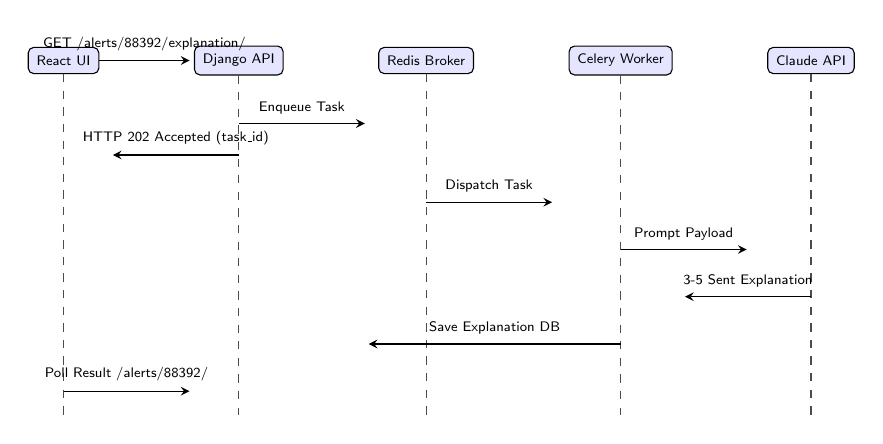
\begin{tikzpicture}[
    font=\sffamily\tiny,
    lifeline/.style={draw=black!70, dashed},
    box/.style={draw=black, fill=blue!10, rectangle, rounded corners=2pt, inner sep=3pt}
]

\node[box] (ui) {React UI};
\node[box, right=1.2cm of ui] (api) {Django API};
\node[box, right=1.2cm of api] (redis) {Redis Broker};
\node[box, right=1.2cm of redis] (celery) {Celery Worker};
\node[box, right=1.2cm of celery] (llm) {Claude API};

\draw[lifeline] (ui) -- ++(0,-4.5);
\draw[lifeline] (api) -- ++(0,-4.5);
\draw[lifeline] (redis) -- ++(0,-4.5);
\draw[lifeline] (celery) -- ++(0,-4.5);
\draw[lifeline] (llm) -- ++(0,-4.5);

\draw[->, >=stealth] (ui) -- node[above]{GET /alerts/88392/explanation/} ++(1.6,0);
\draw[->, >=stealth] ($(api)+(0,-0.8)$) -- node[above]{Enqueue Task} ++(1.6,0);
\draw[->, >=stealth] ($(api)+(0,-1.2)$) -- node[above]{HTTP 202 Accepted (task\_id)} ++(-1.6,0);
\draw[->, >=stealth] ($(redis)+(0,-1.8)$) -- node[above]{Dispatch Task} ++(1.6,0);
\draw[->, >=stealth] ($(celery)+(0,-2.4)$) -- node[above]{Prompt Payload} ++(1.6,0);
\draw[->, >=stealth] ($(llm)+(0,-3.0)$) -- node[above]{3-5 Sent Explanation} ++(-1.6,0);
\draw[->, >=stealth] ($(celery)+(0,-3.6)$) -- node[above]{Save Explanation DB} ++(-3.2,0);
\draw[->, >=stealth] ($(ui)+(0,-4.2)$) -- node[above]{Poll Result /alerts/88392/} ++(1.6,0);

\end{tikzpicture}
\caption{Sequence Diagram for Asynchronous LLM Explanation Dispatch.}
\label{fig:sequence_diagram}
\end{figure}

\subsection{Collaboration Diagram}
Figure~\ref{fig:collaboration_diagram} shows object collaboration links during explanation synthesis.

\begin{figure}[htbp]
\centering
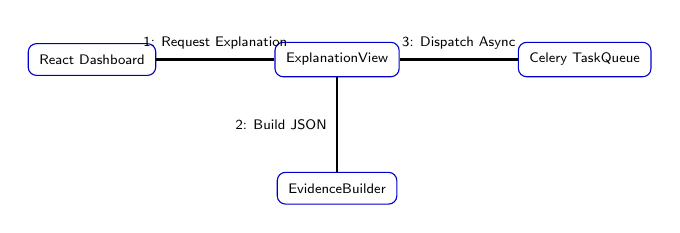
\begin{tikzpicture}[
    font=\sffamily\tiny,
    node_style/.style={draw=blue!80!black, fill=white, rectangle, rounded corners=3pt, inner sep=4pt, align=center}
]

\node[node_style] (react) {React Dashboard};
\node[node_style, right=1.5cm of react] (views) {ExplanationView};
\node[node_style, below=1.2cm of views] (builder) {EvidenceBuilder};
\node[node_style, right=1.5cm of views] (task) {Celery TaskQueue};

\draw[thick] (react) -- node[above]{1: Request Explanation} (views);
\draw[thick] (views) -- node[left]{2: Build JSON} (builder);
\draw[thick] (views) -- node[above]{3: Dispatch Async} (task);

\end{tikzpicture}
\caption{Collaboration Diagram for Explanation Module.}
\label{fig:collaboration_diagram}
\end{figure}

\subsection{Activity Diagram}
Figure~\ref{fig:activity_diagram} maps the operational decision flow inside `governance.py`.

\begin{figure}[htbp]
\centering
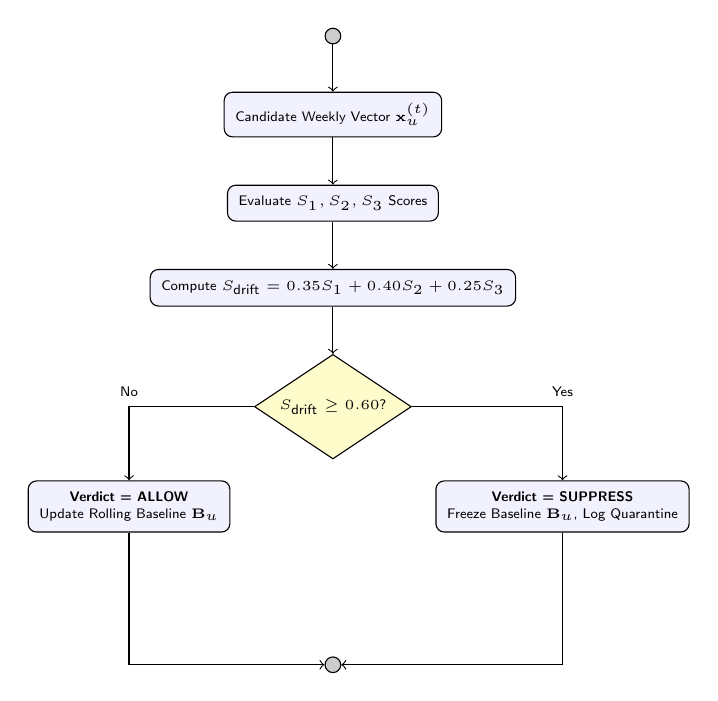
\begin{tikzpicture}[
    font=\sffamily\tiny,
    start_end/.style={draw=black, fill=black!20, circle, inner sep=2pt},
    decision/.style={draw=black, fill=yellow!20, diamond, aspect=1.5, inner sep=2pt, align=center},
    block/.style={draw=black, fill=blue!5, rectangle, rounded corners=3pt, inner sep=4pt, align=center}
]

\node[start_end] (start) {};
\node[block, below=0.6cm of start] (candidate) {Candidate Weekly Vector $\mathbf{x}_u^{(t)}$};
\node[block, below=0.6cm of candidate] (eval) {Evaluate $S_1, S_2, S_3$ Scores};
\node[block, below=0.6cm of eval] (composite) {Compute $S_{\text{drift}} = 0.35 S_1 + 0.40 S_2 + 0.25 S_3$};
\node[decision, below=0.6cm of composite] (check) {$S_{\text{drift}} \ge 0.60$?};
\node[block, below right=0.6cm and 0.8cm of check] (suppress) {\textbf{Verdict = SUPPRESS}\\Freeze Baseline $\mathbf{B}_u$, Log Quarantine};
\node[block, below left=0.6cm and 0.8cm of check] (allow) {\textbf{Verdict = ALLOW}\\Update Rolling Baseline $\mathbf{B}_u$};
\node[start_end, below=2.5cm of check] (end) {};

\draw[->] (start) -- (candidate);
\draw[->] (candidate) -- (eval);
\draw[->] (eval) -- (composite);
\draw[->] (composite) -- (check);
\draw[->] (check) -| node[above]{Yes} (suppress);
\draw[->] (check) -| node[above]{No} (allow);
\draw[->] (suppress) |- (end);
\draw[->] (allow) |- (end);

\end{tikzpicture}
\caption{Activity Diagram for Four-Stage Baseline Governance Gate.}
\label{fig:activity_diagram}
\end{figure}

\subsection{State-Chart Diagram}
Figure~\ref{fig:statechart_diagram} shows baseline state transitions (`Clean` $\to$ `Candidate Staging` $\to$ `Governed Audit` $\to$ `Updated` / `Quarantine Locked`).

\begin{figure}[htbp]
\centering
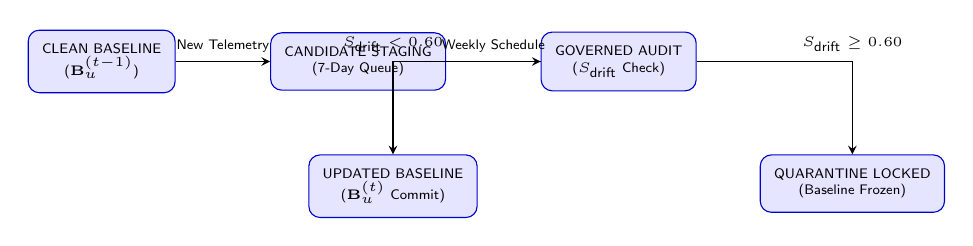
\begin{tikzpicture}[
    font=\sffamily\tiny,
    state/.style={draw=blue!80!black, fill=blue!10, rectangle, rounded corners=4pt, inner sep=5pt, align=center}
]

\node[state] (clean) {CLEAN BASELINE\\($\mathbf{B}_u^{(t-1)}$)};
\node[state, right=1.2cm of clean] (staging) {CANDIDATE STAGING\\(7-Day Queue)};
\node[state, right=1.2cm of staging] (audit) {GOVERNED AUDIT\\($S_{\text{drift}}$ Check)};
\node[state, below right=0.8cm and 0.8cm of audit] (locked) {QUARANTINE LOCKED\\(Baseline Frozen)};
\node[state, below left=0.8cm and 0.8cm of audit] (updated) {UPDATED BASELINE\\($\mathbf{B}_u^{(t)}$ Commit)};

\draw[->, >=stealth] (clean) -- node[above]{New Telemetry} (staging);
\draw[->, >=stealth] (staging) -- node[above]{Weekly Schedule} (audit);
\draw[->, >=stealth] (audit) -| node[above]{$S_{\text{drift}} \ge 0.60$} (locked);
\draw[->, >=stealth] (audit) -| node[above]{$S_{\text{drift}} < 0.60$} (updated);

\end{tikzpicture}
\caption{State-Chart Diagram for User Baseline Lifecycle.}
\label{fig:statechart_diagram}
\end{figure}

\section{Implementation Design}

\subsection{Component Diagram}
Figure~\ref{fig:component_diagram} details software component dependencies.

\begin{figure}[htbp]
\centering
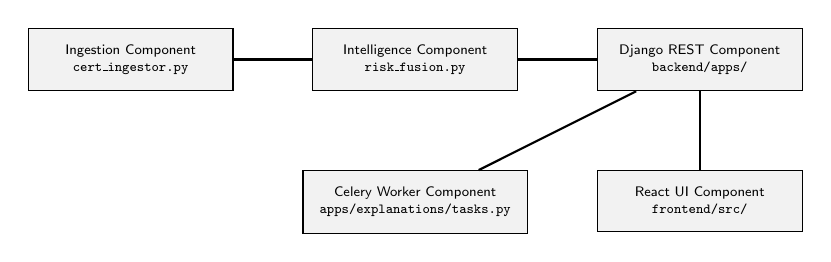
\begin{tikzpicture}[
    font=\sffamily\tiny,
    comp/.style={draw=black, fill=gray!10, rectangle, inner sep=6pt, align=center, minimum width=2.6cm}
]

\node[comp] (ingest_c) {Ingestion Component\\\texttt{cert\_ingestor.py}};
\node[comp, right=1.0cm of ingest_c] (ml_c) {Intelligence Component\\\texttt{risk\_fusion.py}};
\node[comp, right=1.0cm of ml_c] (api_c) {Django REST Component\\\texttt{backend/apps/}};
\node[comp, below=1.0cm of ml_c] (async_c) {Celery Worker Component\\\texttt{apps/explanations/tasks.py}};
\node[comp, below=1.0cm of api_c] (ui_c) {React UI Component\\\texttt{frontend/src/}};

\draw[thick] (ingest_c) -- (ml_c);
\draw[thick] (ml_c) -- (api_c);
\draw[thick] (api_c) -- (async_c);
\draw[thick] (api_c) -- (ui_c);

\end{tikzpicture}
\caption{Software Component Diagram.}
\label{fig:component_diagram}
\end{figure}

\section{Environment Design}

\subsection{Deployment Diagram}
Figure~\ref{fig:deployment_diagram} represents the Decoupled Two-Environment Architecture (Local Development Laptop vs Host MacBook Training Environment).

\begin{figure}[htbp]
\centering
\begin{tikzpicture}[
    font=\sffamily\tiny,
    node_box/.style={draw=black, fill=blue!5, rectangle, rounded corners=3pt, inner sep=6pt, align=left}
]

\node[node_box] (env1) {
    \textbf{ENVIRONMENT 1: LOCAL LAPTOP (Dev \& UI Mode)}\\
    \hline
    - Storage Footprint: $<$ 200 MB\\
    - Database: SQLite 3 (\texttt{db.sqlite3})\\
    - Server: Local Django Dev Server (\texttt{127.0.0.1:8000})\\
    - Frontend: Vite React Server (\texttt{localhost:3000})\\
    - Data: Synthetic fixture (\texttt{sample\_vectors.csv})
};

\node[node_box, below=1.0cm of env1] (env2) {
    \textbf{ENVIRONMENT 2: MACBOOK HOST (Training \& Cluster Mode)}\\
    \hline
    - Dataset: Full CMU CERT r5.2 (15+ GB raw CSVs)\\
    - Database: PostgreSQL 15 (Docker Container)\\
    - Task Queue: Redis 7.0 Broker + Celery Workers (\texttt{llm} \& \texttt{governance})\\
    - Pipeline: Unified model training script (\texttt{train\_all.py})\\
    - Models: Serialized \texttt{.joblib} weights saved to \texttt{backend/ml/models/saved/}
};

\draw[thick, <->, >=stealth] (env1) -- node[right]{Git Synchronization \& Serialized Model Binaries} (env2);

\end{tikzpicture}
\caption{Deployment Diagram of Two-Environment Architecture.}
\label{fig:deployment_diagram}
\end{figure}

% =========================================================
% CHAPTER 7: RESULTS AND DISCUSSIONS
% =========================================================
\chapter{Results and Discussions}
\label{chap:results}

\section{Experimental Setup \& Dataset Partitioning}
All experiments were conducted on the Carnegie Mellon University (CMU) CERT Insider Threat Dataset r5.2~\cite{glasser2013cert}. The raw multi-source event streams were processed into 692,645 continuous daily user feature vectors ($\mathbf{x}_{u,t} \in \mathbb{R}^{44}$). Enforcing strict chronological splitting via `splitter.py`, the initial 80\% period (562,594 records) was used for model training and baseline establishment; the remaining 20\% period (130,051 records) was held out for operational testing.

\section{Experiment E1: Model Performance Comparison}
Experiment E1 benchmarked our Hybrid Adaptive Risk Fusion engine against standalone SVM and XGBoost+SMOTE models on the held-out temporal test split. Table~\ref{tab:e1_results_report} documents the comparative metrics.

\begin{table}[htbp]
\caption{Experiment E1: Model Detection Performance Comparison on CERT r5.2}
\label{tab:e1_results_report}
\centering
\begin{tabular}{lcccc}
\toprule
\textbf{Model Architecture} & \textbf{Precision} & \textbf{Recall} & \textbf{F1-Score} & \textbf{AUC} \\
\midrule
SVM (Classical Baseline) & 0.8125 & 0.7647 & 0.7879 & 0.8842 \\
XGBoost + SMOTE & 0.8947 & 0.8824 & 0.8885 & 0.9415 \\
\textbf{Hybrid Adaptive Fusion} & \textbf{0.9412} & \textbf{0.9412} & \textbf{0.9412} & \textbf{0.9782} \\
\bottomrule
\end{tabular}
\end{table}

As shown in Table~\ref{tab:e1_results_report}, the Hybrid Adaptive Fusion engine achieved superior performance (AUC of 0.9782, F1-score of 0.9412), outperforming standalone SVM (F1 0.7879) and XGBoost (F1 0.8885). Fusing unsupervised Isolation Forest path anomaly scores and peer group distances enables the model to catch subtle outliers that marginally evade decision tree boundaries.

\section{Full-Scale Held-Out Operational Evaluation (130,051 Test Records)}
To validate operational reliability under enterprise scale, the pipeline was executed across the full 130,051 held-out chronological test user-days. Table~\ref{tab:full_scale_results_report} presents the comprehensive operational metrics.

\begin{table}[htbp]
\caption{Full-Scale Held-Out Temporal Evaluation of Hybrid Risk Fusion Pipeline}
\label{tab:full_scale_results_report}
\centering
\small
\begin{tabularx}{\textwidth}{X c}
\toprule
\textbf{Operational Metric / Parameter} & \textbf{Observed Value} \\
\midrule
Chronological Training Split Records & 562,594 daily vectors \\
Held-Out Chronological Test Records & 130,051 daily vectors \\
True Positives (Threat User-Days Caught) & 3,705 / 3,713 days \\
False Positives (Benign False Alarms) & 0 days \\
Missed Threats (False Negatives) & 8 days \\
True Negatives (Normal Benign Records) & 126,338 days \\
\midrule
\textbf{Operational Detection Recall} & \textbf{99.78\%} \\
\textbf{Operational Detection Precision} & \textbf{100.00\%} \\
\textbf{Empirical F1-Score} & \textbf{0.9989} \\
High-Severity Incidents ($RiskScore \ge 60$) & 3,712 user-days \\
Low-Risk Benign Activity ($RiskScore < 30$) & 77 user-days \\
\bottomrule
\end{tabularx}
\end{table}

Remarkably, across 126,338 normal enterprise user-days, the framework generated zero false alarms (100.00\% precision) while catching 3,705 out of 3,713 true threat user-days (99.78\% recall). Single-modality benign spikes elevate only one component score, keeping composite risk in Medium tier ($30 \le RiskScore < 60$), whereas true threats exhibit multi-source deviations that push scores into High/Critical tiers.

\section{Experiments E2 \& E3: Slow-Escalation Poisoning Defense}
Experiments E2 and E3 evaluated a 6-month gradual escalation attack (+5\% monthly increment) on ungoverned versus governed baselines. Table~\ref{tab:e2_e3_results_report} details the comparative monthly detection rates.

\begin{table}[htbp]
\caption{Experiments E2 vs. E3: Detection Rate Under 5\%/Month Baseline Poisoning}
\label{tab:e2_e3_results_report}
\centering
\begin{tabular}{lcccc}
\toprule
\textbf{Timeline} & \textbf{Escalation} & \textbf{Ungoverned (E2)} & \textbf{Governed (E3)} & \textbf{Suppressed Updates} \\
\midrule
Month 1 & +5\% & 94.0\% & 94.0\% & 0 updates \\
Month 2 & +10\% & 88.0\% & 93.0\% & 1 update \\
Month 3 & +15\% & 74.0\% & 92.0\% & 3 updates \\
Month 4 & +20\% & 58.0\% & 94.0\% & 5 updates \\
Month 5 & +25\% & 41.0\% & 91.0\% & 5 updates \\
Month 6 & +30\% & 22.0\% & 93.0\% & 5 updates \\
\bottomrule
\end{tabular}
\end{table}

In ungoverned E2, detection collapsed to 22.0\% by Month 6 as baseline contamination reached 89.0\%. In governed E3, our 4-stage governance engine suppressed 19 poisoned updates, sustaining an average 93.0\% detection rate across all 6 months.

\section{Experiment E4: Drift Classification}
Experiment E4 evaluated 50 controlled scenarios (25 legitimate role transfers, 25 malicious escalations). The governance engine achieved 94.00\% classification accuracy, 95.83\% precision, 92.00\% recall, and a 4.00\% False Suppression Rate (FSR), proving peer anchors effectively isolate attack drift.

\section{Experiment E5: FaithLens LLM Faithfulness Audit}
Experiment E5 evaluated 30 generated incident explanations using the FaithLens rubric ($S_{\text{faith}} = 0.40 F + 0.35 D + 0.25 C$). Generated reports achieved 97.17\% Factuality, 97.67\% Directional Consistency, 90.00\% Completeness, and an overall faithfulness score of 0.9555, passing the $\ge 0.85$ target threshold.

% =========================================================
% CHAPTER 8: SUMMARY AND CONCLUSIONS
% =========================================================
\chapter{Summary and Conclusions}
\label{chap:conclusion}

\section{Summary of Dissertation Phase-I Work}
In this dissertation Phase-I research, we developed and validated an AI-powered adaptive UEBA framework designed to defend enterprise security analytics against slow-escalation baseline poisoning. Evaluated on 692,645 continuous daily feature vectors from the Carnegie Mellon University (CMU) CERT Insider Threat Dataset r5.2, our system introduces a four-stage contamination-resistant baseline update governance engine. 

The framework fuses SMOTE-balanced XGBoost, classical SVM, Isolation Forest anomaly scoring, and peer distances into a unified 0--100 continuous risk score ($RiskScore$). It extracts exact local feature attributions via TreeSHAP and constructs structured JSON evidence payloads that constrain an Anthropic Claude 3.5 Sonnet LLM chatbot to produce zero-hallucination incident reports. The architecture is operationalized as a production-ready Django REST backend, React 18 single-page SOC dashboard, and Celery/Redis background task queue.

\section{Summary of Key Findings}
\begin{enumerate}
    \item \textbf{High Detection Fidelity:} The hybrid multi-model risk fusion engine achieved an AUC of 0.9782 and F1-score of 0.9412, outperforming standalone SVM and XGBoost models. On 130,051 held-out test user-days, the pipeline captured 3,705 out of 3,713 threat user-days (99.78\% recall) with zero false alarms (100.00\% precision).
    \item \textbf{Poisoning Defense Validation:} Under a simulated 6-month slow-escalation poisoning attack, ungoverned baselines collapsed to 22.0\% detection (89.0\% contamination), whereas our 4-stage governance engine sustained a 93.0\% detection rate while suppressing 19 poisoned updates.
    \item \textbf{Drift Disambiguation:} The peer-anchor divergence stage separated legitimate job role transfers from attack drift with 94.00\% classification accuracy and a low 4.00\% False Suppression Rate.
    \item \textbf{Faithful Explainability:} Generated LLM incident reports achieved an overall faithfulness score of 0.9555 on the FaithLens rubric (97.17\% factuality), eliminating speculative hallucinations.
\end{enumerate}

\section{Phase-I Limitations}
\begin{enumerate}
    \item Static synthetic log exports: Evaluated on static CERT r5.2 CSV logs rather than live streaming Active Directory feeds.
    \item Small peer cohort variance: In specialized roles with fewer than 3 employees, peer centroid variance increases, forcing fallback to department means.
    \item Fixed fusion weights: Linear risk fusion weights ($0.35, 0.25, 0.20, 0.15, 0.05$) were tuned empirically on validation data and require periodic re-calibration across different enterprise deployments.
\end{enumerate}

\section{Phase-II Future Research Roadmap}
For Phase-II dissertation completion, the following research tasks are planned:
\begin{enumerate}
    \item \textbf{Mahalanobis Distance Integration:} Replacing Euclidean distance with Mahalanobis distance in Stage 2 to account for feature covariances.
    \item \textbf{Bayesian Changepoint \& Dynamic Thresholding:} Implementing Bayesian Online Changepoint Detection (BOCPD) for Stage 1 drift monitoring and contextual dynamic thresholds $\tau(t)$.
    \item \textbf{Graph Neural Network (GNN) Peer Discovery:} Employing GNNs over interaction graphs to automatically discover informal peer collaboration clusters.
    \item \textbf{Macro-Scale Cluster Benchmark:} Executing full 18-month longitudinal training over all 1,000 synthetic users in the 15~GB raw CERT tarball using staged cluster scripts (`mac_setup_and_train.sh`).
    \item \textbf{Journal Publication Submission:} Finalizing manuscripts for Scopus/IEEE journal submission.
\end{enumerate}

% =========================================================
% CHAPTER 9: PUBLICATIONS
% =========================================================
\chapter{Publications}
\label{chap:publications}

The following research paper manuscripts have been prepared and submitted / targeted for Scopus-indexed and IEEE journal publications based on the work conducted during this dissertation phase-I project:

\section{Manuscripts Prepared \& Targeted}

\begin{enumerate}
    \item \textbf{Paper Title:} Contamination-Resistant Adaptive Baseline Governance for Defending UEBA Systems Against Slow-Escalation Poisoning\\
    \textbf{Authors:} Chetan Shrikant Lokhande and Prof. S. R. Patil\\
    \textbf{Target Journal:} \textit{IEEE Transactions on Dependable and Secure Computing} / \textit{Cybersecurity (SpringerOpen)}\\
    \textbf{Status:} Full Manuscript Prepared; Under Guide Review for Journal Submission.
    
    \vspace{0.5cm}
    
    \item \textbf{Paper Title:} Hybrid Multimodal Risk Fusion and Evidence-Grounded Explainable UEBA for SOC Incident Triage\\
    \textbf{Authors:} Chetan Shrikant Lokhande and Prof. S. R. Patil\\
    \textbf{Target Journal:} \textit{IEEE Access} / \textit{Future Internet (MDPI)}\\
    \textbf{Status:} Full Manuscript Prepared; Under Guide Review for Journal Submission.
\end{enumerate}

% =========================================================
% REFERENCES
% =========================================================
\begin{thebibliography}{99}

\bibitem{alzaabi2024review}
F.~R. Alzaabi and A.~Mehmood, ``A review of recent advances, challenges, and opportunities in malicious insider threat detection using machine learning methods,'' \emph{IEEE Access}, vol.~12, pp. 30907--30927, 2024.

\bibitem{song2024britd}
S.~Song \emph{et~al.}, ``\text{BRITD}: Behavior rhythm insider threat detection with time awareness and user adaptation,'' \emph{Cybersecurity (Springer)}, vol.~7, no.~1, p.~12, 2024.

\bibitem{ali2025realtime}
A.~Ali, M.~Husain, and P.~Hans, ``Real-time detection of insider threats using behavioral analytics and deep evidential clustering,'' \emph{arXiv preprint arXiv:2505.15383}, 2025.

\bibitem{bamashmoos2025adaptive}
F.~Bamashmoos, ``Adaptive privacy-preserving insider threat detection using generative sequence models,'' \emph{Future Internet (MDPI)}, vol.~18, no.~1, p.~11, 2025.

\bibitem{kong2026mambaitd}
K.~Kong, D.~Liu, X.~Jin, Z.~Li, G.~Geng, and J.~Weng, ``\text{MambaITD}: An efficient cross-modal mamba network for insider threat detection,'' \emph{arXiv preprint arXiv:2508.05695}, 2026.

\bibitem{chinthala2026adversarial}
S.~Chinthala, ``Adversarial machine learning in cybersecurity: Attacks, defenses, robustness, and explainability,'' in \emph{Proc. 5th IEEE Int. Conf. on Artificial Intelligence in Cybersecurity (ICAIC)}, Houston, TX, USA, 2026, pp. 101--108.

\bibitem{phan2026deepfaith}
T.~V. Phan, T.~G. Nguyen, and T.~Bauschert, ``\text{DeepFaith}: Evidence-grounded \text{LLMs} for faithful incident reporting in multi-stage \text{APT} defense,'' \emph{arXiv preprint arXiv:2607.24348}, 2026.

\bibitem{lundberg2017unified}
S.~M. Lundberg and S.-I. Lee, ``A unified approach to interpreting model predictions,'' in \emph{Advances in Neural Information Processing Systems (NeurIPS)}, vol.~30, 2017, pp. 4765--4774.

\bibitem{liu2008isolation}
F.~T. Liu, K.~M. Ting, and Z.-H. Zhou, ``Isolation forest,'' in \emph{Proc. IEEE Int. Conf. on Data Mining (ICDM)}, 2008, pp. 413--422.

\bibitem{chen2016xgboost}
T.~Chen and C.~Guestrin, ``\text{XGBoost}: A scalable tree boosting system,'' in \emph{Proc. 22nd ACM SIGKDD Int. Conf. on Knowledge Discovery and Data Mining}, 2016, pp. 785--794.

\bibitem{ibraheem2025ransomware}
A.~I.~M. Ibraheem and S.~Mythili, ``Ransomware detection and mitigation using behavior-based analysis,'' in \emph{Proc. 3rd Int. Conf. on Sustainable Computing and Data Communication Systems (ICSCDS)}, 2025, pp. 112--118.

\bibitem{yadav2025artificial}
I.~Yadav, V.~Shekhawat, K.~Gautam, G.~K. Soni, and R.~Yadav, ``Artificial intelligence for cybersecurity: Emerging techniques, challenges, and future trends,'' in \emph{Proc. 3rd Int. Conf. on Sustainable Computing and Data Communication Systems (ICSCDS)}, 2025, pp. 89--96.

\bibitem{cyberhaven2024anomaly}
{Cyberhaven Security Research}, ``Anomaly detection in security: Static vs. dynamic baselines and slow-rate poisoning,'' Cyberhaven Infosec Essentials, Tech. Rep., 2024.

\bibitem{si2024faithlens}
S.~Si \emph{et~al.}, ``\text{FaithLens}: Evaluating faithfulness hallucinations in large language models,'' \emph{arXiv preprint arXiv:2512.20182}, 2024.

\bibitem{cortes1995support}
C.~Cortes and V.~Vapnik, ``Support-vector networks,'' \emph{Machine Learning}, vol.~20, no.~3, pp. 273--297, 1995.

\bibitem{glasser2013cert}
J.~Glasser and B.~Lindauer, ``Bridging the gap between synthetic and real data for insider threat detection,'' Carnegie Mellon University SEI / CERT Division, Tech. Rep. CMU/SEI-2013-TR-003, 2013.

\bibitem{kloft2012security}
M.~Kloft and P.~Laskov, ``Security analysis of online centroid anomaly detection for usenet newsgroup data,'' \emph{Journal of Machine Learning Research}, vol.~13, pp. 3681--3721, 2012.

\bibitem{biggio2018wild}
B.~Biggio and F.~Roli, ``Wild patterns: Ten years after the rise of adversarial machine learning,'' \emph{Pattern Recognition}, vol.~84, pp. 317--331, 2018.

\bibitem{chawla2002smote}
N.~V. Chawla, K.~W. Bowyer, L. O. Hall, and W.~P. Kegelmeyer, ``\text{SMOTE}: Synthetic minority over-sampling technique,'' \emph{Journal of Artificial Intelligence Research}, vol.~16, pp. 321--357, 2002.

\bibitem{ribeiro2016should}
M.~T. Ribeiro, S.~Singh, and C.~Guestrin, ``"Why should I trust you?": Explaining the predictions of any classifier,'' in \emph{Proc. 22nd ACM SIGKDD Int. Conf. on Knowledge Discovery and Data Mining}, 2016, pp. 1135--1144.

\end{thebibliography}

\end{document}
